\section{Results on Controlled Data}
\label{sec:results}

\subsection{Detection and closure-time baselines (RQ1, RQ2)}
Over the 5 catalog scenarios analysed in one shared database,
SAT-SA emitted every declared finding family (true positives 5, false
negatives 0) and 7 undeclared families: micro precision
0.417, recall 1.000, F1 0.588. The recommended supervisory
action matched the declared action in 4 of 5
scenarios. Precision depends on database layout: analysed one scenario per database
(A01), the full worker set reached 0.556, because cross-entity
workers in a shared database see other scenarios' records.

On 12 construction-labelled critical closures (3 fast),
SAT-SA's fast-closure detector, a fixed threshold and a MAD rule each reached F1
1.00; z-score and IQR rules found none (recall
0.0); seeded random reached 0.33.
\emph{The detector ties simple baselines and offers no detection advantage on this
corpus.}

\subsection{Prioritization against simple baselines (RQ2)}
Across 20 generated populations, SAT-SA placed a median
0.800 of the pathological entities in its top 20\% and needed a
median of 7.0 reviews to find all of them (Table~\ref{tab:prio},
Fig.~\ref{fig:prio}). Its recall@20\% exceeded random order in all
20 populations (median paired difference
0.59, 95\% bootstrap 0.41 to
0.60) and alert-volume ranking in all 20
(0.40; 0.30 to 0.60).
\emph{Against the fastest-median-closure heuristic the comparison is mixed}: higher in
8, equal in 11 and lower in
1 populations (median difference 0.00,
interval 0.00 to 0.20); SAT-SA needed fewer reviews
in 12 populations and more in 6.

These results must be read against how the data were made. The populations come from
SAT-SA's own generator, whose pathological profile deliberately injects the behaviours
that SAT-SA's detector families target. Because the generated populations inject
behaviours targeted by SAT-SA's detector families, PR01 is a controlled sensitivity
and ranking-mechanism evaluation rather than an unbiased benchmark of general
supervisory effectiveness: it characterizes how the ranking responds under these
generated conditions. Even under this favourable construction, a single closure-speed rule captures most of the separation.

\begin{table}[t]
\caption{Prioritization on 20 generated populations of
20 entities (5 pathological): medians over
populations (PR01). Volume = reviews needed to find all pathological entities.}
\label{tab:prio}
\centering
\scriptsize
\begin{tabular}{@{}lrrrrr@{}}
\toprule
Ranking & P@10\% & R@20\% & NDCG@20\% & NDCG@30\% & Volume \\
\midrule
SAT-SA ($P_e$) & 1.000 & 0.800 & 1.000 & 0.869 & 7.0 \\
Fastest median closure & 1.000 & 0.600 & 0.832 & 0.837 & 11.5 \\
Critical/high alert volume & 0.500 & 0.200 & 0.246 & 0.318 & 18.0 \\
Random (mean of permutations) & 0.245 & 0.201 & 0.248 & 0.276 & 17.5 \\
\bottomrule
\end{tabular}
\end{table}


\begin{figure}[!htbp]
\centering
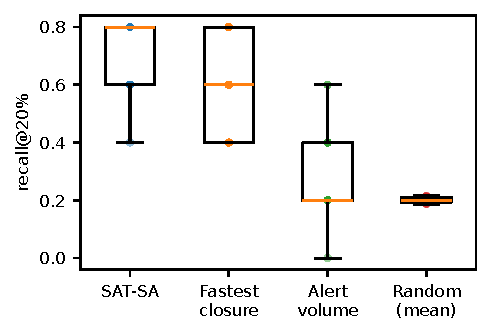
\includegraphics[width=0.5\linewidth]{figures/fig-prioritization.pdf}
\caption{Recall@20\% of generator-labelled pathological entities across
20 generated populations (PR01). The generator injects behaviours that
SAT-SA targets, so this is a controlled mechanism test, not an unbiased benchmark.}
\label{fig:prio}
\end{figure}

\subsection{One-worker ablation (RQ2)}
Removing one of the 16 workers at a time (Table~\ref{tab:ablation}),
fast-closure and negative-space carried recall on the catalog (0.600
and 0.600 without them; 1.000 with all workers).
Removing recurrence-without-remediation or coverage-gap \emph{raised} precision because
those workers emitted only undeclared families here. On five generated populations
(exploratory), mean recall@20\% was 0.760 with all workers and rose to
0.800 without the anomaly, recurrence, coverage-gap or
workflow-reconstruction worker, whereas removing the peer-benchmark or case-similarity
worker lowered it to 0.720. On these populations, therefore, some
workers add ranking noise to the measured metric.

We read this nuanced result narrowly. The full worker set spans a broader analytical
signal space than the generated populations exercise, and the ranking objective is
specific to the generator's pathological profile. The ablation therefore shows that
some workers can reduce this particular metric on these populations; worker utility
is task- and population-dependent (Section~\ref{sec:threats}).

\begin{table}[t]
\caption{One-worker ablation (A01): catalog micro precision/recall (5
scenarios, one database per scenario) and mean population recall@20\% (Pop.\ R@20; five seeds,
exploratory). Only workers whose removal changed a value are listed; ``--'' = unchanged from the full set.}
\label{tab:ablation}
\centering
\scriptsize
\begin{tabular}{@{}L{5.4cm}rrr@{}}
\toprule
Workers & Precision & Recall & Pop.\ R@20 \\
\midrule
All 16 & 0.556 & 1.000 & 0.760 \\
$-$ fast closure & 0.429 & 0.600 & 0.600 \\
$-$ negative space & 0.500 & 0.600 & 0.640 \\
$-$ evidence completeness & 0.500 & 0.800 & -- \\
$-$ recurrence without remediation & 0.714 & 1.000 & 0.800 \\
$-$ coverage gap & 0.625 & 1.000 & 0.800 \\
$-$ anomaly & -- & -- & 0.800 \\
$-$ workflow reconstruction & -- & -- & 0.800 \\
$-$ peer benchmark & -- & -- & 0.720 \\
$-$ case similarity & -- & -- & 0.720 \\
\bottomrule
\end{tabular}
\end{table}


\subsection{Imperfect evidence (RQ3)}
Each perturbed condition declared its family, affected records and expected validation
outcome before it ran, on a fresh tenant database. Validation matched the declared
contract in 245 of 245 conditions with an expectation
(Table~\ref{tab:robust}): malformed timestamps, chronology violations, missing columns
and duplicates with native identifiers were rejected. Two behaviours limit
interpretation (Fig.~\ref{fig:robust}). First, validation is all-or-nothing:
independent omission of records left dangling references and rejected the whole
submission in 3, 11 and
14 of 25 replicates at 10, 25 and 50\% omission, whereas
referentially consistent omission was never rejected and changed the emitted finding
families in 1, 11 and 15
replicates. Second, \emph{stale and contradictory evidence is accepted silently}: all
15 conditions with records outside the assessment period were
accepted without warning and without any change to findings or risk, and contradictory
dispositions or a closed case with an open alert produced no finding. SAT-SA
implements no period, recency or cross-record consistency validation.

\begin{table}[t]
\caption{Imperfect-evidence conditions by family (R01b). Rejected = whole submission
rejected by validation; changed = emitted finding families differed from the paired
control; ``--'' = no condition rejected (all analysed). Validation matched its declared contract in 245 of
245 conditions with an expectation.}
\label{tab:robust}
\centering
\scriptsize
\begin{tabular}{@{}lrrrr@{}}
\toprule
Family & Conditions & Rejected & Analysed & Findings changed \\
\midrule
Missingness & 173 & 33 & 140 & 43 \\
Duplication & 34 & 25 & 9 & 5 \\
Malformation & 15 & 15 & 0 & 0 \\
Conflict & 18 & 5 & 13 & 4 \\
Staleness (no expectation) & 15 & -- & 15 & 0 \\
Control & 5 & -- & 5 & 0 \\
\bottomrule
\end{tabular}
\end{table}


\begin{figure}[!htbp]
\centering
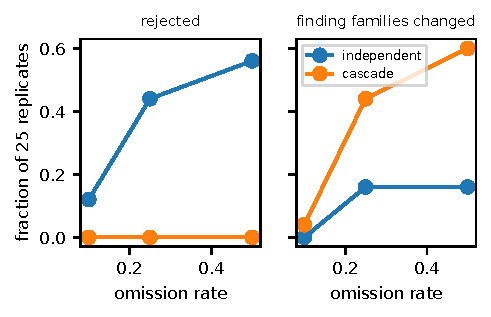
\includegraphics[width=0.55\linewidth]{figures/fig-robustness.pdf}
\caption{Record omission (R01b): independent omission is often rejected by
all-or-nothing validation; referentially consistent omission is accepted and changes
findings more often as the rate grows.}
\label{fig:robust}
\end{figure}

\subsection{Peer-cohort sensitivity (RQ4)}
Over 96 engineered cells (Fig.~\ref{fig:peer}), cohorts of two peers never
produced a finding, as Eq.~\eqref{eq:peer} requires three. With a tight cohort spread,
7 of eight subject values were flagged from three peers upward---every
value except the one at the cohort median. With a wide spread only extreme slow
subjects were flagged at small cohorts (2 at three peers), and fast
subjects only from five peers upward as the MAD narrowed (4 at five
peers). The peer rule is therefore sensitive to cohort size and dispersion: small or
heterogeneous cohorts miss deviations, and tight cohorts flag small ones.

\begin{figure}[!htbp]
\centering
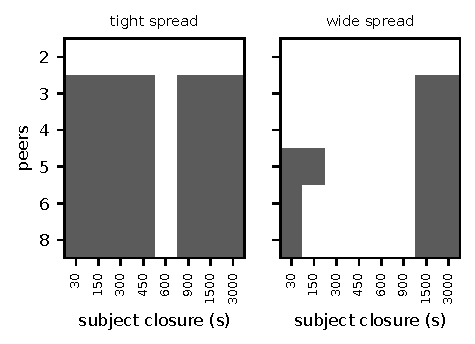
\includegraphics[width=0.68\linewidth]{figures/fig-peer.pdf}
\caption{Peer findings by cohort size, spread and subject closure value; dark cells
emitted a finding (P01, 96 cells).}
\label{fig:peer}
\end{figure}

\subsection{Orchestration cost and recovery (RQ5)}
On one machine with SQLite, 30 paired trials per mode gave median processing
times, excluding the human decision, of 1.276\,s (direct),
1.433\,s (LangGraph) and 0.976\,s (unreviewed benchmark
mode) (Table~\ref{tab:orch}). LangGraph minus direct was a median 0.096\,s
per workflow (95\% bootstrap \ensuremath{-}0.020 to 0.211\,s; the
interval includes zero), with 38 more database statements and
7 checkpoints per run; findings and risk were identical across modes
in every trial. Review with finalization added a median 0.318\,s over
unreviewed processing; finalization took 0.288\,s and receipt
verification 0.062\,s. Interruptions were injected at 6
points in both modes with 3 trials per cell: transient failures and
simulated crashes during analysis, before recommendations, at a worker restart during
review, and during finalization. \emph{In the evaluated interruption scenarios},
36 of 36 runs recovered, 36 with outputs
identical to the uninterrupted reference; completed stages were repeated
0 times, and every run had exactly one decision, one finalization and a
verifying receipt. Real process kills, network partitions and database failover were
not exercised.

\begin{table}[!htbp]
\caption{Orchestration cost on one machine with SQLite (O01, 30 paired
trials per mode; the human decision excluded). Median and p95 in seconds; Outside =
seconds outside the domain stages; DB = database statements. Graph $-$ direct: median
0.096\,s, 95\% bootstrap \ensuremath{-}0.020 to 0.211\,s
(graph slower in 19 of 30 pairs). Finalization took
0.288\,s, receipt verification 0.062\,s and run and
finding attestation 0.853\,s (medians).}
\label{tab:orch}
\centering
\small
\setlength{\tabcolsep}{4pt}
\begin{tabular}{@{}L{4.2cm}rrrr@{}}
\toprule
Mode & Median & p95 & Outside & DB \\
\midrule
Direct (reviewed) & 1.276 & 2.010 & 0.055 & 420 \\
LangGraph (reviewed) & 1.433 & 2.206 & 0.115 & 458 \\
Unreviewed benchmark mode & 0.976 & 1.655 & 0.029 & 253 \\
\bottomrule
\end{tabular}
\end{table}


\subsection{Integrity of the decided record (RQ6)}
On one finalized controlled workflow, each of 14 mutations was applied,
verified, restored and re-verified (Table~\ref{tab:trust}). Verification detected
13 of 13 mutations of signed state---decision action and
reason, finding, risk, recommendation, observation scope, source provenance,
submission record payload, artifact digest, canonical payload, receipt signature,
receipt public key and ledger chain---while the negative control (1
mutation of an unsigned operational queue field) still verified, as designed. These
results cover the tested mutation classes on one workflow; verification detects
alteration after the fact rather than preventing it (Section~\ref{sec:system}).

\begin{table}[!htbp]
\caption{Integrity mutation matrix on one finalized workflow (T01): 13
of 13 mutations of signed state detected; the unsigned control still
verified. Full targets are in the supplementary material.}
\label{tab:trust}
\centering
\small
\setlength{\tabcolsep}{4pt}
\begin{tabular}{@{}L{7.4cm}ll@{}}
\toprule
Mutated element & Expected & Observed \\
\midrule
Decision action; decision reason & tampered & tampered \\
Finding rationale; observation scope & tampered & tampered \\
Risk profile; recommendation & tampered & tampered \\
Source provenance; submission record payload & tampered & tampered \\
Artifact digest; canonical payload & tampered & tampered \\
Receipt signature; receipt public key & tampered & tampered \\
Ledger chain (predecessor hash) & tampered & tampered \\
Unsigned queue field (control) & verified & verified \\
\bottomrule
\end{tabular}
\end{table}

